% Options for packages loaded elsewhere
\PassOptionsToPackage{unicode}{hyperref}
\PassOptionsToPackage{hyphens}{url}
%
\documentclass[
  ignorenonframetext,
]{beamer}
\usepackage{pgfpages}
\setbeamertemplate{caption}[numbered]
\setbeamertemplate{caption label separator}{: }
\setbeamercolor{caption name}{fg=normal text.fg}
\beamertemplatenavigationsymbolsempty
% Prevent slide breaks in the middle of a paragraph
\widowpenalties 1 10000
\raggedbottom
\setbeamertemplate{part page}{
  \centering
  \begin{beamercolorbox}[sep=16pt,center]{part title}
    \usebeamerfont{part title}\insertpart\par
  \end{beamercolorbox}
}
\setbeamertemplate{section page}{
  \centering
  \begin{beamercolorbox}[sep=12pt,center]{section title}
    \usebeamerfont{section title}\insertsection\par
  \end{beamercolorbox}
}
\setbeamertemplate{subsection page}{
  \centering
  \begin{beamercolorbox}[sep=8pt,center]{subsection title}
    \usebeamerfont{subsection title}\insertsubsection\par
  \end{beamercolorbox}
}
\AtBeginPart{
  \frame{\partpage}
}
\AtBeginSection{
  \ifbibliography
  \else
    \frame{\sectionpage}
  \fi
}
\AtBeginSubsection{
  \frame{\subsectionpage}
}

\usepackage{amsmath,amssymb}
\usepackage{iftex}
\ifPDFTeX
  \usepackage[T1]{fontenc}
  \usepackage[utf8]{inputenc}
  \usepackage{textcomp} % provide euro and other symbols
\else % if luatex or xetex
  \usepackage{unicode-math}
  \defaultfontfeatures{Scale=MatchLowercase}
  \defaultfontfeatures[\rmfamily]{Ligatures=TeX,Scale=1}
\fi
\usepackage{lmodern}
\ifPDFTeX\else  
    % xetex/luatex font selection
\fi
% Use upquote if available, for straight quotes in verbatim environments
\IfFileExists{upquote.sty}{\usepackage{upquote}}{}
\IfFileExists{microtype.sty}{% use microtype if available
  \usepackage[]{microtype}
  \UseMicrotypeSet[protrusion]{basicmath} % disable protrusion for tt fonts
}{}
\makeatletter
\@ifundefined{KOMAClassName}{% if non-KOMA class
  \IfFileExists{parskip.sty}{%
    \usepackage{parskip}
  }{% else
    \setlength{\parindent}{0pt}
    \setlength{\parskip}{6pt plus 2pt minus 1pt}}
}{% if KOMA class
  \KOMAoptions{parskip=half}}
\makeatother
\usepackage{xcolor}
\newif\ifbibliography
\setlength{\emergencystretch}{3em} % prevent overfull lines
\setcounter{secnumdepth}{-\maxdimen} % remove section numbering


\providecommand{\tightlist}{%
  \setlength{\itemsep}{0pt}\setlength{\parskip}{0pt}}\usepackage{longtable,booktabs,array}
\usepackage{calc} % for calculating minipage widths
\usepackage{caption}
% Make caption package work with longtable
\makeatletter
\def\fnum@table{\tablename~\thetable}
\makeatother
\usepackage{graphicx}
\makeatletter
\newsavebox\pandoc@box
\newcommand*\pandocbounded[1]{% scales image to fit in text height/width
  \sbox\pandoc@box{#1}%
  \Gscale@div\@tempa{\textheight}{\dimexpr\ht\pandoc@box+\dp\pandoc@box\relax}%
  \Gscale@div\@tempb{\linewidth}{\wd\pandoc@box}%
  \ifdim\@tempb\p@<\@tempa\p@\let\@tempa\@tempb\fi% select the smaller of both
  \ifdim\@tempa\p@<\p@\scalebox{\@tempa}{\usebox\pandoc@box}%
  \else\usebox{\pandoc@box}%
  \fi%
}
% Set default figure placement to htbp
\def\fps@figure{htbp}
\makeatother
% definitions for citeproc citations
\NewDocumentCommand\citeproctext{}{}
\NewDocumentCommand\citeproc{mm}{%
  \begingroup\def\citeproctext{#2}\cite{#1}\endgroup}
\makeatletter
 % allow citations to break across lines
 \let\@cite@ofmt\@firstofone
 % avoid brackets around text for \cite:
 \def\@biblabel#1{}
 \def\@cite#1#2{{#1\if@tempswa , #2\fi}}
\makeatother
\newlength{\cslhangindent}
\setlength{\cslhangindent}{1.5em}
\newlength{\csllabelwidth}
\setlength{\csllabelwidth}{3em}
\newenvironment{CSLReferences}[2] % #1 hanging-indent, #2 entry-spacing
 {\begin{list}{}{%
  \setlength{\itemindent}{0pt}
  \setlength{\leftmargin}{0pt}
  \setlength{\parsep}{0pt}
  % turn on hanging indent if param 1 is 1
  \ifodd #1
   \setlength{\leftmargin}{\cslhangindent}
   \setlength{\itemindent}{-1\cslhangindent}
  \fi
  % set entry spacing
  \setlength{\itemsep}{#2\baselineskip}}}
 {\end{list}}
\usepackage{calc}
\newcommand{\CSLBlock}[1]{\hfill\break\parbox[t]{\linewidth}{\strut\ignorespaces#1\strut}}
\newcommand{\CSLLeftMargin}[1]{\parbox[t]{\csllabelwidth}{\strut#1\strut}}
\newcommand{\CSLRightInline}[1]{\parbox[t]{\linewidth - \csllabelwidth}{\strut#1\strut}}
\newcommand{\CSLIndent}[1]{\hspace{\cslhangindent}#1}

\makeatletter
\@ifpackageloaded{caption}{}{\usepackage{caption}}
\AtBeginDocument{%
\ifdefined\contentsname
  \renewcommand*\contentsname{Table of contents}
\else
  \newcommand\contentsname{Table of contents}
\fi
\ifdefined\listfigurename
  \renewcommand*\listfigurename{List of Figures}
\else
  \newcommand\listfigurename{List of Figures}
\fi
\ifdefined\listtablename
  \renewcommand*\listtablename{List of Tables}
\else
  \newcommand\listtablename{List of Tables}
\fi
\ifdefined\figurename
  \renewcommand*\figurename{Figure}
\else
  \newcommand\figurename{Figure}
\fi
\ifdefined\tablename
  \renewcommand*\tablename{Table}
\else
  \newcommand\tablename{Table}
\fi
}
\@ifpackageloaded{float}{}{\usepackage{float}}
\floatstyle{ruled}
\@ifundefined{c@chapter}{\newfloat{codelisting}{h}{lop}}{\newfloat{codelisting}{h}{lop}[chapter]}
\floatname{codelisting}{Listing}
\newcommand*\listoflistings{\listof{codelisting}{List of Listings}}
\makeatother
\makeatletter
\makeatother
\makeatletter
\@ifpackageloaded{caption}{}{\usepackage{caption}}
\@ifpackageloaded{subcaption}{}{\usepackage{subcaption}}
\makeatother

\usepackage{bookmark}

\IfFileExists{xurl.sty}{\usepackage{xurl}}{} % add URL line breaks if available
\urlstyle{same} % disable monospaced font for URLs
\hypersetup{
  pdftitle={The Radical Right and the Politicization of Climate Policy},
  pdfauthor={Zach Dickson},
  hidelinks,
  pdfcreator={LaTeX via pandoc}}


\title{The Radical Right and the Politicization of Climate Policy}
\subtitle{Presentation for UCD School of Politics and International
Relations}
\author{Zach Dickson}
\date{}
\institute{(co-authored with Sara Hobolt)London School of Economics}

\begin{document}
\frame{\titlepage}


\begin{frame}{Motivation}
\phantomsection\label{motivation}
\begin{itemize}[<+->]
\item
  \textbf{Climate change} is a pressing global issue
\item
  \textbf{Political consensus} on the need for action
\item
  But implementation remains contentious
\item
  \begin{quote}
  Despite growing consensus on the need for climate action,
  implementation remains politically contentious. \textbf{Why?}
  \end{quote}
\end{itemize}
\end{frame}

\begin{frame}
\begin{block}{The Radical Right and Climate Change}
\phantomsection\label{the-radical-right-and-climate-change}
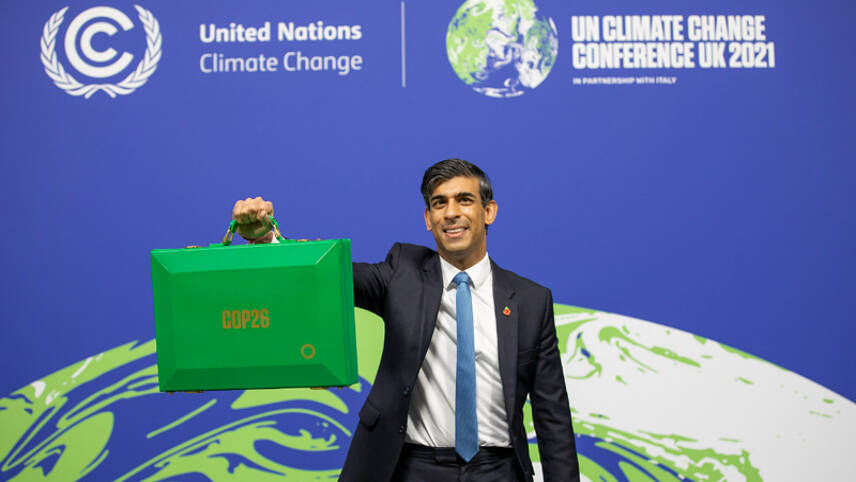
\includegraphics[width=5.20833in,height=3.64583in]{images/rishi_green.png}


\includegraphics[width=4.16667in,height=2.60417in]{images/green_libdems.png}

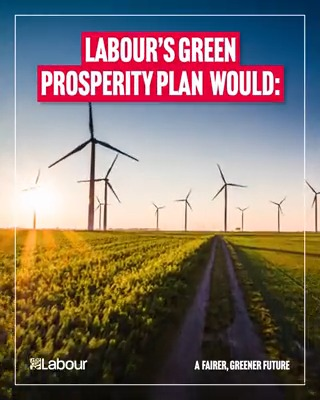
\includegraphics[width=3.64583in,height=4.16667in]{images/labour_prosperity.png}

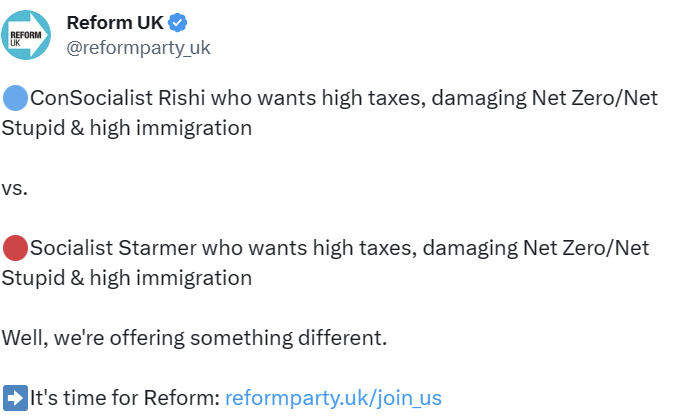
\includegraphics[width=6.77083in,height=4.6875in]{images/reform_uk.png}
\end{block}
\end{frame}

\begin{frame}{Party Competition and Wedge Issue Politics}
\phantomsection\label{party-competition-and-wedge-issue-politics}
\begin{itemize}[<+->]
\item
  \textbf{Party competition} is central to understanding policy outcomes
\item
  Parties compete on \textbf{issue ownership} and
  \textbf{entrepreneurship}
\item
  Issue owners are widely recognized as \textbf{experts} on the issue
\item
  Entrepreneurial parties seek to \textbf{change the status quo} by
  politicizing new issues
\item
  \begin{quote}
  \textbf{Argument:} Radical right parties are politicizing climate
  change as a wedge issue to divide mainstream coalitions.
  \end{quote}
\end{itemize}
\end{frame}

\begin{frame}{Climate Change as a Wedge Issue}
\phantomsection\label{climate-change-as-a-wedge-issue}
\begin{itemize}[<+->]
\tightlist
\item
  Three key elements:

  \begin{itemize}[<+->]
  \tightlist
  \item
    \textbf{Issue attention}

    \begin{itemize}[<+->]
    \tightlist
    \item
      RR parties increase salience of climate issues
    \end{itemize}
  \item
    \textbf{Adversarial positioning}

    \begin{itemize}[<+->]
    \tightlist
    \item
      RR parties take an oppositional stance on climate policy
    \end{itemize}
  \item
    \textbf{Mobilizing potential}

    \begin{itemize}[<+->]
    \tightlist
    \item
      A significant share of voters hold sceptical views of climate
      change policies
    \end{itemize}
  \end{itemize}
\end{itemize}
\end{frame}

\begin{frame}{Expectations}
\phantomsection\label{expectations}
\begin{itemize}[<+->]
\tightlist
\item
  Increase in \textbf{salience} of climate issues for radical right
  parties
\item
  RR parties will take an \textbf{adversarial position} on climate
  policy
\item
  A significant share of voters who \emph{do not already} support the RR
  hold \textbf{sceptical views}
\end{itemize}
\end{frame}

\begin{frame}{Research Design \& Methods}
\phantomsection\label{research-design-methods}
\begin{itemize}[<+->]
\tightlist
\item
  \textasciitilde500k Party Press Releases from 76 parties (2010-2022)

  \begin{itemize}[<+->]
  \tightlist
  \item
    Includes over 50k press releases from radical right parties
  \end{itemize}
\item
  European Social Survey data
\item
  UK and German Election Study Panel Data
\item
  \textbf{Text analysis} to measure salience and adversarial positioning

  \begin{itemize}[<+->]
  \tightlist
  \item
    Train and validate language models for:
  \item
    \href{https://huggingface.co/z-dickson/CAP_multilingual}{Text
    classification}
  \item
    \href{https://huggingface.co/z-dickson/bart-large-cnn-climate-change-summarization}{Generative
    summarization}
  \end{itemize}
\end{itemize}
\end{frame}

\begin{frame}{Party Press Releases}
\phantomsection\label{party-press-releases}
\begin{center}
\pandocbounded{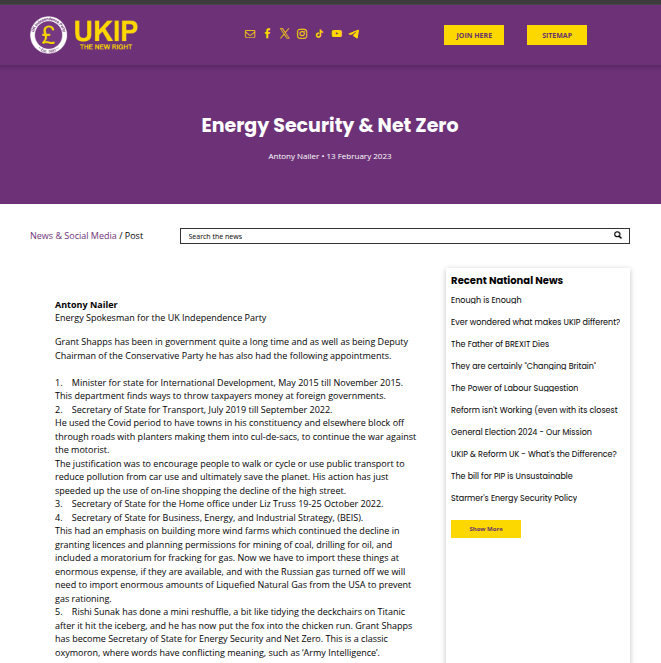
\includegraphics[keepaspectratio]{images/ukip_press_release.png}}
\end{center}
\end{frame}

\begin{frame}{Results: Salience}
\phantomsection\label{results-salience}
\begin{quote}
Radical right parties are increasingly focusing on climate issues
\end{quote}

\begin{center}
\pandocbounded{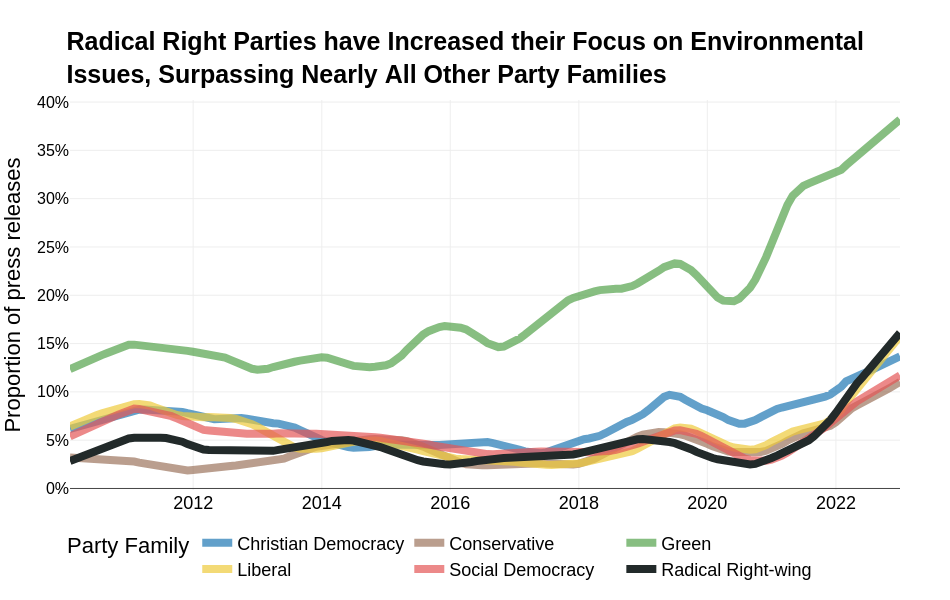
\includegraphics[keepaspectratio]{images/figure1.png}}
\end{center}
\end{frame}

\begin{frame}{Results: Adversarial Position}
\phantomsection\label{results-adversarial-position}
\begin{quote}
Radical right parties are uniquely oppositional on climate issues
\end{quote}

\begin{center}
\pandocbounded{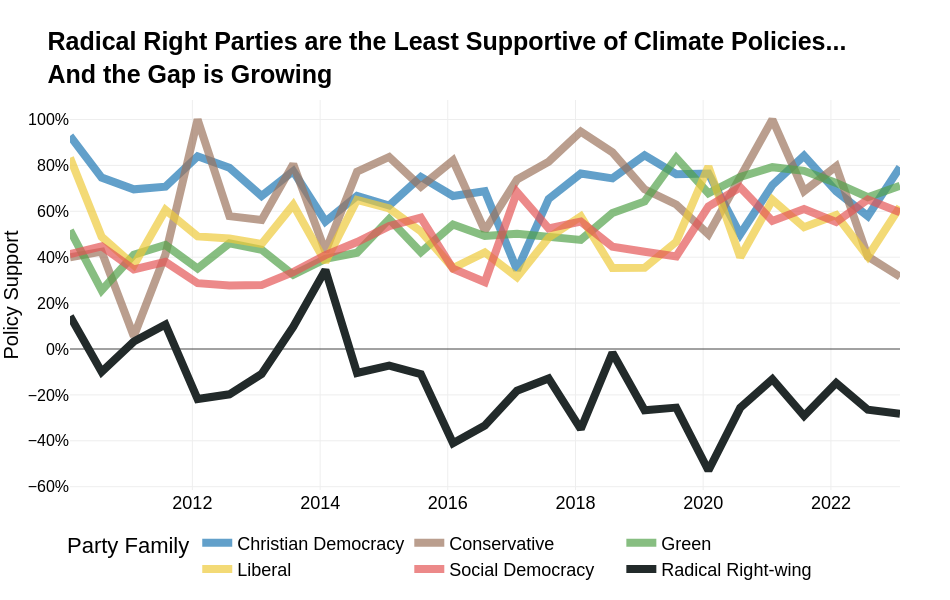
\includegraphics[keepaspectratio]{images/figure2.png}}
\end{center}
\end{frame}

\begin{frame}{Results: Mobilizing Potential}
\phantomsection\label{results-mobilizing-potential}
\begin{quote}
A significant share of voters across parties hold sceptical views
\end{quote}

\begin{center}
\pandocbounded{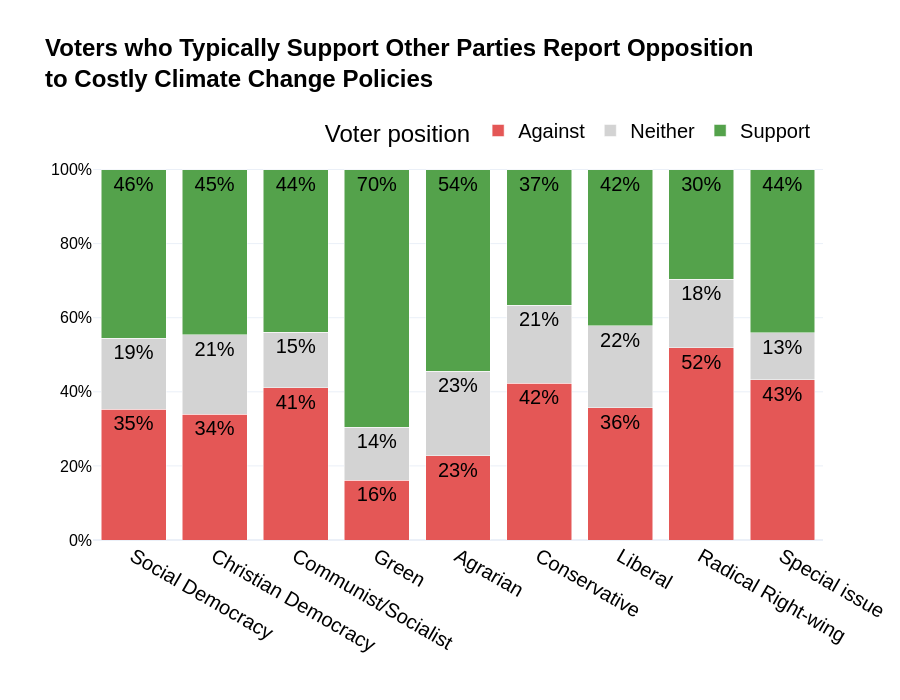
\includegraphics[keepaspectratio]{images/figure3.png}}
\end{center}
\end{frame}

\begin{frame}{Vote Switching}
\phantomsection\label{vote-switching}
\begin{quote}
Radical right parties are mobilizing voters
\end{quote}

\begin{center}
\pandocbounded{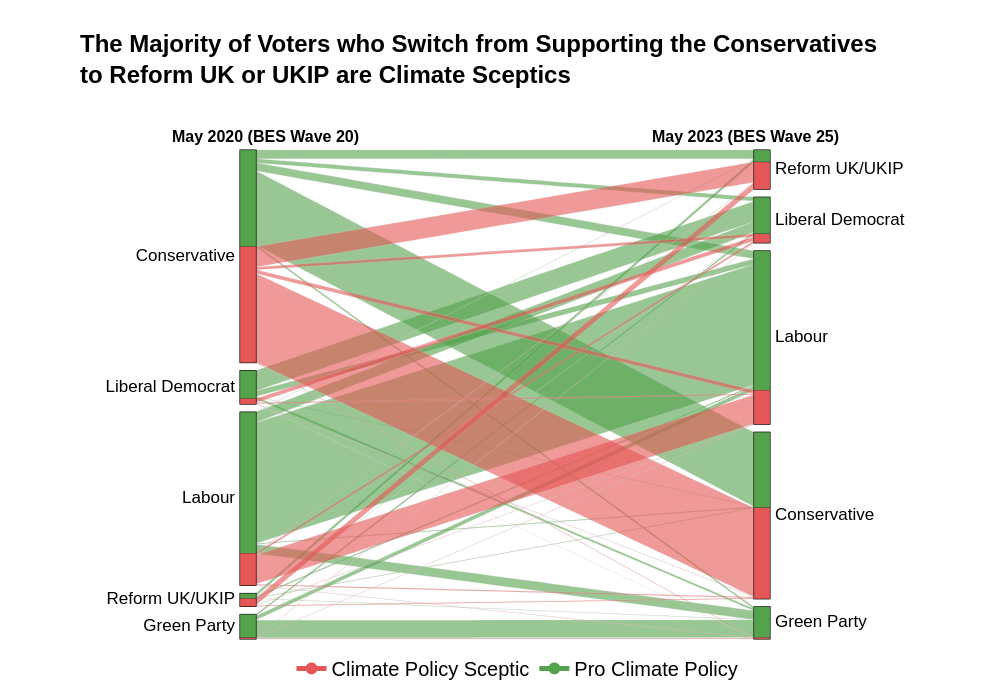
\includegraphics[keepaspectratio]{images/figure7.png}}
\end{center}
\end{frame}

\begin{frame}{Discussion}
\phantomsection\label{discussion}
\begin{itemize}[<+->]
\tightlist
\item
  Climate change is a \textbf{wedge issue} that divides mainstream
  coalitions
\item
  Radical right parties are increasingly \textbf{politicizing} climate
  change

  \begin{itemize}[<+->]
  \tightlist
  \item
    Increasing salience
  \item
    Taking adversarial positions
  \item
    Mobilizing voters
  \end{itemize}
\end{itemize}
\end{frame}

\begin{frame}{Implications for Mainstream Parties}
\phantomsection\label{implications-for-mainstream-parties}
\begin{itemize}[<+->]
\tightlist
\item
  \textbf{Address the Distributional Consequences of Climate Policy}

  \begin{itemize}[<+->]
  \tightlist
  \item
    Climate action must be socially fair. Failure to address the costs
    for lower- and middle-income groups risks backlash and opens space
    for radical-right mobilization.
  \end{itemize}
\item
  \textbf{Communicate Climate Policy in Terms of Security, Sovereignty,
  and Stability}

  \begin{itemize}[<+->]
  \tightlist
  \item
    Reframe climate action not as sacrifice, but as a protection of
    national economic and social resilience---especially to counter
    nationalist narratives.
  \end{itemize}
\item
  \textbf{Build Broader, Cross-Cutting Coalitions for Climate Action}

  \begin{itemize}[<+->]
  \tightlist
  \item
    Parties should proactively engage non-traditional climate
    constituencies---rural voters, working-class communities, small
    businesses---to increase ownership and reduce vulnerability to wedge
    strategies and radical right parties.
  \end{itemize}
\end{itemize}
\end{frame}

\begin{frame}{Thank You!}
\phantomsection\label{thank-you}
\begin{itemize}
\tightlist
\item
  \textbf{Contact:}
  \href{mailto:z.dickson@lse.ac.uk}{\nolinkurl{z.dickson@lse.ac.uk}}
\item
  \textbf{Article:} Dickson \& Hobolt (2024).
  \href{https://journals.sagepub.com/doi/10.1177/00104140241271297}{Going
  Against the Grain: Climate Change as a Wedge Issue for the Radical
  Right}. \emph{Comparative Political Studies}
\end{itemize}

\begin{center}
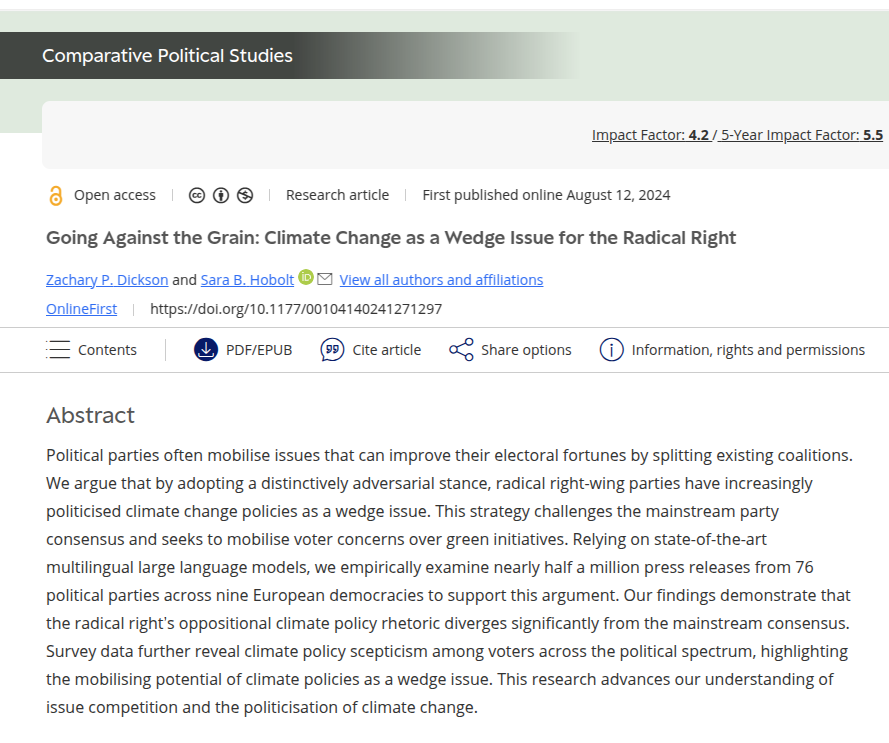
\includegraphics[width=0.5\linewidth,height=\textheight,keepaspectratio]{images/CPS_abstract.png}
\end{center}
\end{frame}

\begin{frame}{References}
\phantomsection\label{references}
\phantomsection\label{refs}
\begin{CSLReferences}{0}{1}
\end{CSLReferences}
\end{frame}




\end{document}
